\section{译者补充:经典电磁理论下的光学基础}\label{sec:译者补充:经典电磁理论下的光学基础}
\begin{remark}
    本节内容不是原书内容,而是译者根据《Optics》\citep{hecht2016optics}
    补充并参考\citet{OpticsChinese}翻译的,请酌情参考和斧正。
    本节内容只简要介绍相关基础概念和结论,
    并不像正式的物理和光学教材那样严谨,请读者批判性地看待本节内容。
    本节要求读者具备较好的微积分与电磁理论知识储备。
    此外读者需注意,本节遵循有关内容惯例采用右手坐标系,
    与正文pbrt采用的左手坐标系不同。
\end{remark}

\subsection{波动}\label{sub:波动}
光的本质是什么?光是波动现象还是粒子现象?
这个问题非常复杂。早在二十世纪,物理学家们就已经发现,
光的电磁理论的经典结论在微观层级上完全不成立。
然而当我们站在通常的大尺度视角下,电磁波及其经典理论已经够用了。
为了打好基础,我们从波的数学描述说起,它也适用于一切物理波。

\subsubsection*{一维波}
行进中的\keyindex{波}{wave}{}的一个本质特性是,
它是传播波的\keyindex{介质}{medium}{}的自持\keyindex{扰动}{disturbance}{}。
\keyindex{机械波}{mechanical wave}{wave\ 波}是
我们最熟悉的波,如琴弦上的波、液体表面的波、
空气中的\keyindex{声波}{sound wave}{wave\ 波}以及固体和流体中的压缩波。
\begin{definition}[\keyindex{纵波}{longitudinal wave}{wave\ 波}]
    介质在波动方向上位移。
\end{definition}
\begin{definition}[\keyindex{横波}{transverse wave}{wave\ 波}]
    介质位移的方向垂直于波动方向。
\end{definition}
\begin{example}
    声波是纵波;琴弦上的波、电磁波是横波。
\end{example}
波区别于粒子流的几个关键特征之一是,
扰动在前进,但实物介质并不前进。
就像风吹起滚滚麦浪,但麦穗只是原地摇摆。
\begin{figure}[htbp]
    \centering
    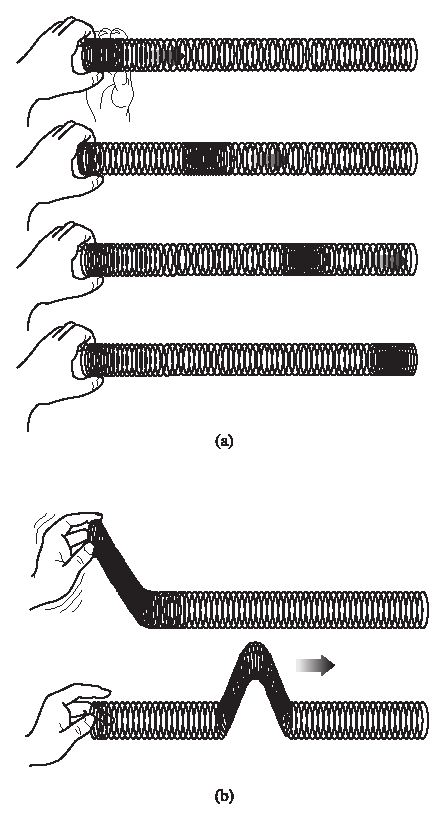
\includegraphics[width=0.6\linewidth]{Pictures/chap08/longitudinalAndTransverseWave.eps}
    \caption{弹簧中的(a)纵波;(b)横波。}
    \label{fig:08ex02.0201}
\end{figure}

我们暂不追究扰动的本质,而专注研究描述波动的方程应该具备怎样的形式。
设某个这样的扰动$\psi$以恒定速度$v$沿正$x$方向运动。
既然扰动在运动,则它必然是位置和时间的函数:
\begin{align}
    \psi(x,t)=f(x,t)\, ,
\end{align}
其中$f(x,t)$对应于某个具体函数或波形。
如\reffig{08ex02.0203}(a)所示,一个脉冲在静止坐标系$S$中以速度$v$运动。
我们取定任意时刻$t$即可得到那个时刻波的\keyindex{剖面}{profile}{},
就像脉冲经过时给它“拍照”。例如$t=0$有
\begin{align}
    \psi(x,t)\bigg|_{t=0}=f(x,0)=f(x)
\end{align}
表示0时刻波的剖面。

现在,我们先只考虑传播时形状不变的波。
在一段时间$t$后,脉冲沿$x$轴前进了距离$vt$,其余不变。
如\reffig{08ex02.0203}(b),我们引入新坐标系$S'$并与脉冲以相同速度$v$运动。
则在该坐标系中$\psi$不再是时间的函数,而是静止不变的剖面,即
\begin{align}
    \psi=f(x')\, ,
\end{align}
这意味着坐标系$S'$中的扰动在任意时刻$t$的形状,
都和$S$中$t=0$时两者具有同一原点时扰动的形状相同,如\reffig{08ex02.0203}(c)所示。
为了将上式改写为$S$中某静止观察者描述的形式,我们利用
\begin{align}
    x'=x-vt
\end{align}
得到
\begin{align}
    \psi(x,t)=f(x-vt)\, .
\end{align}
上式是一维\keyindex{波函数}{wave function}{wave\ 波}的最一般形式。
它描述了一个具有所需剖面形状$f(x)$的波,它以速度$v>0$沿正$x$方向运动。
相似地,如果波向负$x$方向运动,则上式应改写为
\begin{align}
    \psi(x,t)=f(x+vt)\, .
\end{align}
总之变量$x$和$t$一定作为一个整体变量$x\mp vt$出现。

\begin{figure}[htbp]
    \centering
    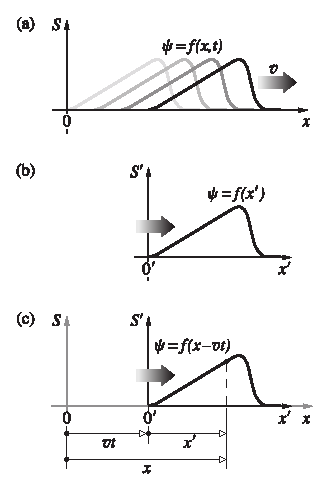
\includegraphics[width=0.5\linewidth]{Pictures/chap08/MovingReferenceFrame.eps}
    \caption{运动参考系。}
    \label{fig:08ex02.0203}
\end{figure}

\subsubsection*{波动微分方程}
接下来我们推导一维波动方程的形式。